% 
% Annual Cognitive Science Conference
% Sample LaTeX Paper -- Proceedings Format
% 

% Original : Ashwin Ram (ashwin@cc.gatech.edu)       04/01/1994
% Modified : Johanna Moore (jmoore@cs.pitt.edu)      03/17/1995
% Modified : David Noelle (noelle@ucsd.edu)          03/15/1996
% Modified : Pat Langley (langley@cs.stanford.edu)   01/26/1997
% Latex2e corrections by Ramin Charles Nakisa        01/28/1997 
% Modified : Tina Eliassi-Rad (eliassi@cs.wisc.edu)  01/31/1998
% Modified : Trisha Yannuzzi (trisha@ircs.upenn.edu) 12/28/1999 (in process)
% Modified : Mary Ellen Foster (M.E.Foster@ed.ac.uk) 12/11/2000
% Modified : Ken Forbus                              01/23/2004
% Modified : Eli M. Silk (esilk@pitt.edu)            05/24/2005
% Modified : Niels Taatgen (taatgen@cmu.edu)         10/24/2006
% Modified : David Noelle (dnoelle@ucmerced.edu)     11/19/2014
% Modified : Roger Levy (rplevy@mit.edu)     12/31/2018



%% Change "letterpaper" in the following line to "a4paper" if you must.

\documentclass[10pt,letterpaper]{article}

\usepackage{cogsci}
\usepackage{color}
%\cogscifinalcopy % Uncomment this line for the final submission 
\usepackage{tikz}
\usetikzlibrary{bayesnet}
\usepackage{amsmath,amssymb,amsfonts,amsthm}
\usepackage{pgfplotstable}
\usepackage{csvsimple}
\usepackage{booktabs}

\usepackage{pslatex}
\usepackage{apacite}
\usepackage{float} % Roger Levy added this and changed figure/table
                   % placement to [H] for conformity to Word template,
                   % though floating tables and figures to top is
                   % still generally recommended!

%\usepackage[none]{hyphenat} % Sometimes it can be useful to turn off
%hyphenation for purposes such as spell checking of the resulting
%PDF.  Uncomment this block to turn off hyphenation.


%\setlength\titlebox{4.5cm}
% You can expand the titlebox if you need extra space
% to show all the authors. Please do not make the titlebox
% smaller than 4.5cm (the original size).
%%If you do, we reserve the right to require you to change it back in
%%the camera-ready version, which could interfere with the timely
%%appearance of your paper in the Proceedings.

\definecolor{Red}{RGB}{255,0,0}
\definecolor{Green}{RGB}{10,200,100}
\definecolor{Blue}{RGB}{10,100,200}
\definecolor{Orange}{RGB}{255,153,0}

\newcommand{\denote}[1]{\mbox{ $[\![ #1 ]\!]$}}
\newcommand*\diff{\mathop{}\!\mathrm{d}}
\newcommand{\red}[1]{\textcolor{Red}{#1}}  
\newcommand{\mht}[1]{\textcolor{Blue}{[mht: #1]}}  

\title{How many observations is one generic worth?}
 
\author{{\large \bf M. H. Tessler^{1} (tessler@mit.edu)}, {\large \bf Sophie Bridgers^{2} (sbridge@stanford.edu)}, and {\large \bf Joshua B. Tenenbaum^{1} (jbt@mit.edu)} \ \\
  ^{1}Department of Brain and Cognitive Sciences, MIT \\
    ^{2}Department of Psychology, Stanford University}


\begin{document}

\maketitle


\begin{abstract}
Include no author information in the initial submission, to facilitate
blind review.  The abstract should be one paragraph, indented 1/8~inch on both sides,
in 9~point font with single spacing. The heading ``{\bf Abstract}''
should be 10~point, bold, centered, with one line of space below
it. This one-paragraph abstract section is required only for standard
six page proceedings papers. Following the abstract should be a blank
line, followed by the header ``{\bf Keywords:}'' and a list of
descriptive keywords separated by semicolons, all in 9~point font, as
shown below.

\textbf{Keywords:} 
add your choice of indexing terms or keywords; kindly use a
semicolon; between each term
\end{abstract}


\section{Introduction}

The world is a confusing and confounding place, but the right kind of generalizations allow us to navigate the world with ease.
We come to know these generalizations either by learning from experience or by learning from others.
Indeed, infants and young children draw strong generalizations from just a few examples \red{(cite devo/infant research}).
When these examples are presented in a pedagogical manner---via an act intended by another agent to change the learner's beliefs---stronger generalizations are often drawn \red{(cite: butler, ...)}. 
But generalizations can also be conveyed with language, using what is called \emph{generic language} (or, \emph{generics}; e.g., \emph{Swans are white}) \red{(cite: Carlson, Leslie, Tessler}).
What is the relationship between learning from language and learning from experience, between inductive generalizations drawn from observations (either those presented pedagogically vs. not) and those learned from generics?
In particular, how many observations is one generic worth?

%We understand the lightning tends to strike tall objects and that smoking causes cancer, but how do we come to know these generalizations?

Articulating the precise relationship between learning from examples and learning from language is difficult because learning from linguistic utterances operates via the linguistic message's \emph{truth conditions}, which are often difficult to specify:
The meanings of even the simplest linguistic expressions can change dramatically depending on the context and the content. 
Generics are a clear case of this context-specificity:  while \emph{Triangles have three sides} should be taken to mean that exactly 100\% of triangles have three sides, \emph{Swans are white} is more tolerating of exceptions (i.e., there are black swans); \emph{Mosquitos carry malaria} is an example of a generic that conveys a very weak generalization: the vast majority of real-world mosquitos do not carry the virus. 
Despite this heterogeneity, \cite{Tessler2019psychrev} proposed a Bayesian formulation to understanding generics, where a generic acts as a \emph{vague quantifier}, \emph{a la} \emph{some}, \emph{most}, \emph{all} but in which the truth functional threshold for a generic is underspecified or vague; that is, whereas \emph{most} can be literally taken to mean \emph{more than half} and \emph{all} literally means 100\%, the threshold for a generic is not specified \emph{a priori}, but is determined in context.
This model of generics as a kind of vague quantifier bears an intruiging relationship to models of belief-updating from observations: With some minimal assumptions, a generic updates beliefs in a way analogous to a single, pedagogically-presented example \cite{Tessler2020genint}. 

The idea that a generic may in some way be analogous to a single, pedagogically-presented example was developed independently by  \citeA{Csibra2015}, trying to understand infant cognition. 
The main idea is that because infants conceive of objects as instances of kinds, pedagogical reference to an individual can act as a symbolic reference to the kind. 
Then, any demonstration that may result in this pedagogical episode would be understood as predicating the kind, and hence, a kind of non-verbal generic.

Thus, proposals from two rather different theoretical frameworks---Bayesian models of semantics and infant cognitive development---point to the hypothesis that a generic might be equivalent to a single, pedagogically-sampled example.\footnote{Of course, the pedagogical context must signal an event wherein the teacher is aiming to inform the learner about the category and not, say, about a special member of the category. We return to this point in the Discussion.}
On the other hand, the relationship between generics and pedagogical examples that \citeA{Csibra2015} proposes for preverbal infants may not be the same throughout development; indeed, 3- and 4-year-olds can interpret the ostensive cue of pointing as a signal that the information conveys is not generalizable, but specific to the examplars referenced by her point \cite{meyer2013}.
Furthermore, the prediction from the vague quantifier model of generics is contingent on the assumption that the prior distribution over possible, truth-functional thresholds is uniform (i.e., a generic, in the abstract, could carry any quantificational strength, and all are equally likely \emph{a priori}); if that prior distribution is instead skewed towards higher thresholds (e.g., a generic, in the abstract, is more likely to imply \emph{most} than imply \emph{some}), then it would be worth a larger number of examples. 

%That is, while cognitive scientists for a long time have been concerned with the precise computations that underly learning from examples---most prominently explored in a Bayesian setting these days---and even how difficult sampling assumptions of those examples (i.e., a learner assuming a pedagogically sampling rule) can strengthen this belief updating mechanism, learning from language has received comparatively little attention. 


%There are two suggestions for how learning from examples might relate to learning from generics.
%The first is derived via the comptuational model of \cite{Tessler2019psychrev}: We show how the vague quantifier model relates to Bayesian belief-updating from observations. 
%Under the most minimal of assumptions, the literal listener component of   \cite{Tessler2019psychrev}reduces to belief-updating given a \emph{single, positive example} and the pragmatic listener model introduced by  \cite{Tessler2020genint} would amount to a belief-updating model given a pedagogically presented single example.


We take an empirical approach to investigate the relationship between learning from examples and learning from generic language.
We develop an empirical paradigm where participants can learn about a novel category either from examples or from language and ask them to judge the likelihood that a future instance of a category would have the property \cite<cf.,>{gelman2003; cimpian2010; brandone2014; tessler2020genint}.
We titrate the number of examples participants learn in order to determine the point at which the strength of the generalization implied by examples is equal to the strength of the generalization implied by a generic statement. 
We find that, contra the theoretical proposals out in the literature, a generic is worth about three, pedagogically sampled examples. 
The implications of this relationship, as well as its potential context-sensitivity and development, are discussed.



\section{Theoretical Background}

We highlight two proposals in the literature concerning the precise relationship of learning from observations and learning from generics.  The first comes from computational cognitive science, and in particular, the model of generic language as a vague quantifier proposed by Tessler2019. The second comes from cognitive development and in particular a view of infants' understanding of objects and kinds proposed by Csibra2015. 

\subsection{Generics as vague quantifier}

Tessler2019 proposed a Bayesian model for understanding generic language by drawing on the tools of truth-functional semantics and treating a generic as a kind of vague quantifier.
The truth conditions of quantifiers can be formalized as threshold functions on the property prevalence (e.g., $\denote{some} = p > 0$; $\emph{most}= p > 0.5$; $\denote{all} = p = 1$). The model is similar in their truth conditions---$\denote{\emph{gen}} = p > \theta$---but treats the  
semantic threshold variable as underspecified in the semantics but inferred in context. Formally, their model puts a probability distribution over the threshold variable---$\theta \sim P(\theta)$---following format treatment of gradable adjectives like \emph{tall} \red{(cite Lassiter)}. Combining this underspecified, threshold semantics with the prior knowledge a listener would bring to the table $P(x)$ yields the following model of generic interpretation
$$
L(x, \theta) \propto P(x) P(\theta) \delta_{x > \theta}
$$

The prior distribution $P(x)$ is an object of theoretical interest in its own right and has been investigated extensively in the original presentation of this model \red{(cite Tessler2019, Tessler2020)}. 
Of particular interest for our purposes is a mathematical relationship pointed out Tessler2020, which can be seen by integrating out the listener's uncertainty about the threshold variable. 

\mht{insert math}

What we see here is that the original model of Tessler2019 can be reformulated in terms of belief-updating from observations. 
The exact number of observations depends upon the prior distribution over the semantic threshold $P(\theta)$.  
Tessler2019 used a uniform prior $\theta \sim Uniform(0,1)$ (i.e, \emph{a priori}, anything could count as a true generic, without regard to the actual prevalence of the feature).
Integrating out the threshold using this prior yields a model of belief-updating given a single example. 

It is important to note that this relationship is only manifested at the level of a literal listener.
Tessler2020 argue that the strength of generic interpretation should be understood not as a literal listener interpretation but as a pragmatic interpretation of a weak semantics (see also \red{vanRooij2019} for a similar argument). 
If this is the case, we would expect a generic to be equivalent to a single, pragmatically-enriched (or, pedagogically understood) example. 


\subsection{Non-verbal generics}

A second proposal for the relationship between belief updating from generic language and belief updating from observations comes from \citeA{Csibra2015}. Csibra argues that preverbal infants view objects as instances of kinds. That is, when observing an instance of a novel category (call it a \emph{blicket}), they not only have the capacity to individuate this object as a singular entity (i.e., \emph{this is a blicket}) but also have the capacity to see the object as an index to the kind (i.e., \emph{this blicket is a pointer to the kind \textsc{blickets}}) .  When an object is presented to an infant with ostensive, pedagogical cues (a la \emph{natural pedagogy} \cite{CsibraGereley}), the infant will interpret the object, not as a singular entity, but as an index to the kind; then, if a property is predicated (i.e., demonstrated) of that object (e.g., the blicket is shown to squeak), it will be taken by the infant to apply to the kind. That is, the pedagogical demonstration will be understood as a (non-verbal) generic: \emph{Blickets squeak}. Thus, this account draws a direct connection between generics and a single, pedagogical example. \footnote{It should be noted that the account of \citeA{Csibra2015} is intended to be applied to infant cognition. There is no direct or indirect link proposed for this view to be applied to adult cognition or even the cognition of young children who have acquired their first language. \red{In fact, there may be empirical bases to believe this account would not apply to cognition broadly (Baldwin ...).} Thus, this argument should be understood as an application of the account of \citeA{Csibra2015} and not a direct theoretic consequence of it.} 

\section{Experiment}

\subsection{Method}

\subsubsection{Participants}

We recruited \red{XXX} adult participants from Amazon's Mechanical Turk. 
Participants were restricted to those with U.S. IP addresses with at least a 95\% work approval rating. 
In addition, participants were required to pass a simple language comprehension test that we deployed in order to weed out bots and other bad-faith participants. 
The test involved a sentence in which a named speaker (e.g., Joseph) says to a named listener (e.g., Elizabeth) ``It's a beautiful day, isn't it?''. 
Participants were asked to type in a text box to whom the speaker (in this case: Joseph) is talking (i.e., Elizabeth).
Speaker and listener names were randomized in a way that could not be read off the source .html file.
Participants were given three attempts to correctly identify the listener. 
If they did not succeed within 3 attempts, they would be unable to proceed with the experiment.
Since participants who fail this check are required to exit the experiment before completing the task, we do not have an estimate for how many participants fail this check. 

\subsubsection{Materials}

We used exemplars from four, semi-novel natural categories and one artifact category.
The basic-level categories from which our novel categories were created were birds, bugs, fish, and flowers. 
The instances presented in a category had the same general physical features but each example had a unique shape, size, and color that was randomly sampled from an underlying distribution with relatively small variance (i.e., the examples were heterogeneous, but tightly clustered in perceptual space).

The feature to be learned for all categories was presented auditorally. 
The features are shown in Table 1. 

\subsubsection{Procedure}

Participants competed three trials. 

\subsection{Behavioral results}


\begin{figure}[t]
\begin{center}
\includegraphics[width=\linewidth]{figs/genex-pilots_10conditions_reordered.pdf}
\end{center}
\caption{Experiment results}
\label{fig:results}
\end{figure}

\mht{trial order effects?}

\mht{item effects?}


\subsection{Bayesian data analysis}

We approach the question of how many observations one generic is worth from a Bayesian perspective. 
We formalize this question by asking when the distribution of responses for a given experimental condition is more likely to come from the same distribution of responses for the generic condition than from a different distribution. 

\begin{figure}[ht]
  \begin{center}
    \begin{tabular}{cc}
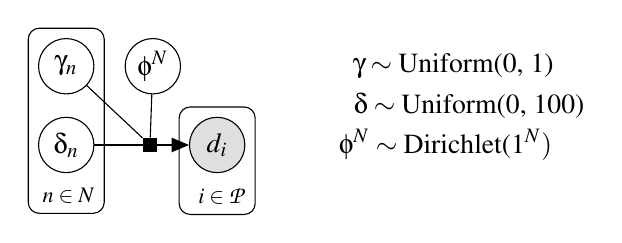
\begin{tikzpicture}

  \node[obs]          (d)   {$d_i$}; %
  \node[latent, left=0.1cm of d, yshift=1cm] (mx) {$\boldsymbol{\phi}^N$} ; %
  \node[latent, left=1.2cm of d, yshift=1cm]  (sx) {$\gamma_n$} ; %
  \node[latent, left=1.2cm of d, yshift=0cm]  (dx) {$\delta_n$} ; %
  \factor[left=of d] {x-f} {} {mx,sx,dx} {d} ; %

\plate{data} {
(d)
}{$i \in \mathcal{P}$};

\plate{mix} {
(sx)(dx)
}{$n \in N$};

\node[] at (3,1.0) {$\gamma \sim \text{Uniform(0, 1)}$};
\node[] at (3.2,0.5) {$\delta \sim \text{Uniform(0, 100)}$};
\node[] at (2.9,0) {$\boldsymbol{\phi}^N \sim \text{Dirichlet(}\boldsymbol{1}^N)$};


\end{tikzpicture}

    \end{tabular}
  \end{center}
  \caption{Bayesian data analysis model for a single experimental condition. Individual responses ($d_i$) for all participants $\mathcal{P}$ are assumed to be generated by a mixture of Beta distributions. Each Beta is parameterized by a mean $\gamma_n$ and concentration (or, inverse-variance) $\delta_n$ parameter. The number of mixture components is given by $N$. Priors over parameters are shown on the right. This model is repeated for each experimental condition.}
  \label{fig:bayesnet}
\end{figure}


In order to characterize the distribution of responses in each of the experimental conditions, we first perform a Bayesian analysis to determine the best function that characterizes our response variable, since they are clearly not normally distributed.
Since the slider bar ratings we acquire are values between 0 and 1, we assume the distribution of responses is a mixture of some number of Beta distributions (which have support defined over 0 and 1).\footnote{The Beta distribution is defined over the open interval (0, 1), whereas our response variable could contain the endpoints 0 and 1. To accommodate responses that are exactly 0 or exactly 1, we adjust these end-point responses to be equal to 0.001 and 0.999, respectively.}
We fit the data with either a single Beta distribution, a mixture of two Betas, or a mixture of three Betas, with a new mixture for each condition independently (Figure \ref{fig:bayesnet}). 
We compute Bayes Factors by comparing the marginal likelihood of the data under each hypothesis about the number of mixture components ($N = \{1, 2, 3\}$).
We find that the data is much more likely to come from a mixture of Beta distributions than a single distribution, though the data is inconclusive as to whether or not it is a mixture of two distributions or of three (Table~\ref{tab:componentBF}). 
Since the data is inclusive between two- and three- mixture components, we use a mixture of two distributions to characterize the responses for computational simplicity. 


\begin{center}
  \begin{table}[h]
    \centering
    \pgfplotstabletypeset[sci zerofill,
    col sep = comma,
    every head row/.style={before row = \toprule, after row = \midrule},
    every last row/.style={after row = \bottomrule},
    columns/Model Comparison/.style={string type, column name={Comparison}, column type = l},
    columns/bf/.style={column name={Bayes Factor}, dec sep align},
    columns/logbf/.style={column name={log BF}, sci sep align, sci}]
    {output_from_r/n_component_bf.csv}
    \caption{Bayes Factors comparing different linking functions for the experimental data.}
    \label{tab:componentBF}
  \end{table}
\end{center}


Having determined the best linking function for the distribution of responses, we perform a Bayesian analysis to determine which---if any---of the results of our experimental conditions is equivalent to the results of the generic-only condition. 
We do this by computing the marginal likelihood of the combined data set of the generic condition plus one of the other experimental conditions under the assumption that they are generated from the same distribution (i.e., the same two-component mixture-of-Betas model). 
We compare this likelihood to that calculated by assuming the two conditions were generated by independent distributions (i.e, two different two-component mixture-of-Beta distributions). 
The comparison of these marginal likelihoods gives us the Bayes Factor quantifying the evidence in support of the hypothesis that two conditions were generated from the same underlying distribution (i.e., the generic is worth n observations). 
The results are shown in Table \ref{tab:nobsBF}).



\begin{center}
  \begin{table}[h]
    \centering
    \pgfplotstabletypeset[sci zerofill,
    col sep = comma,
    every head row/.style={before row = \toprule, after row = \midrule},
    every last row/.style={after row = \bottomrule},
    columns/condition/.style={string type, column name={Comparison}, column type = l},
    columns/bf/.style={column name={Bayes Factor}, dec sep align},
    columns/logbf/.style={column name={log BF}, sci sep align}]
    {output_from_r/n_obs_bf.csv}
    \caption{Bayes Factors in support of the hypothesis that the strength of generalization implied by a generic is equal to that of the experimental condition.}
    \label{tab:nobsBF}
  \end{table}
\end{center}






\section{Discussion}

Successfully navigating the environment requires anticipating what is to come, and abstract generalizations allow us to reason flexibly about instances of categories and events that we have not yet experienced. 
These generalizations can be constructed both by directly observing instances in the world and by being told the generalization in the form of a generic sentence. 
But what is the relationship between learning from examples and learning from generics? 
Here we ask a simple question: How many observations is one generic worth?
We find that, contra extant theoretical proposals, the strength of the generalization implied by a generic is equivalent to roughly three pedagogically-sampled examples. 

\subsection{Generics about other predicates}

In our experiment, we used predicates that are directly observable---sounds that an animal or object could make---and that could plausibly be construed as idiosyncratic properties of individuals (e.g., \emph{This fep squawks}) or characteristic properties of categories (e.g., it is typical of feps to squawk).
Observing different kinds of properties in general should lead to different strengths of generalization implied by examples \cite{Nisbett1983}. 
Does this imply that the examples---generics exchange rate is different for generalizing different properties?
Not necessarily.
It is also the case that the strength of generalization implied by a generic varies by the type of property \cite{Tessler2020}. 
In fact, it is a prediction of the theory of \citeA{Tessler2019, Tessler2020} that the exchange rate will be the same across properties. (What is different across properties, according to the Tessler2019, is the prior knowledge.)

\subsection{Generics about superordinate categories}

In our experiment, we used novel categories that would plausibly be construed as subordinate level categories.
We focus on subordinate level categories to isolate the contribution of the number of examples without concern as to the differences or variability among the examples with respect to the extension of the category.
That is, the examples--generics exchange rate will, in general, depend upon the level of abstraction of the category. 
Learning from examples the same kind of generalization as that conveyed with a generic about a superordinate category (e.g., \emph{Mammals are worm-blooded}) will be much more difficult than the subordinate categories we used. 
In particular, to make a strong generalization to the category of mammals, a learner would benefit from a diverse set of examples (e.g., bears, cats, whales, ...) and significantly benefited from the prior knowledge that different animal families have a consistent kind of bloodedness. 
The power of generics then scales with the level of abstraction of the category: Generics about more abstract, superordinate categories will, in general, be harder to learn from examples than generics about basic level or subordinate level categories. 

\subsection{Relationship to children}

\mht{Changes from infancy to early childhood?}

\mht{Changes across childhood?}

\subsection{Relation to other tasks}

Our experiment method is similar but distinct from other studies investigating the interpretation of generics vis a vis examples or statistics.
\citeA{Cimpian2010} compared the strength of generalization implied by a generic (what they called \emph{implied prevalence}) to the statistics of the feature in terms of its prevalence in the category that led participants to endorse the generic (what they call \emph{truth conditions}). They found that generics (at least, generics about the kinds of predicates they tasted) tend to be interpreted more strongly than what one would expect given the statistical information that lead people to endorse generics. 

\citeA{Kushnir2016} examined the strength of generalizations and trust in informants after jointly hearing generic language and observing some number relevant instances of the category with/without the property (e.g., hearing \emph{Blickets squeak} and then observing 2 out of 10 blickets squeak.
This paradigm is a little direct measure of the number of the observations that a single generic is worth because it incorporates the additional variable of trust in testimony.
That is, a learner can explain away conflicting observations and testimony through two means: (a) weakening the generalization strength implied by the generic (e.g., \emph{the speaker did not mean most the property but only some}) and (b) weakening trust in the speaker (e.g., \emph{the speaker was ill-informed}). 
This interplay between the vagueness of generics and speaker trust is a complex problem that should receive more attention on its own right. 

\subsection{Other limitations of this study}

One other limitation of our paradigm that we wish to highlight is that our paradigm does not evoke uninhibited, automatic, bonafide communicative reasoning but rather is embedded in a story book that depicts certain communicative acts \red{(cite Clark?)}. 
For example, the incidental condition is not really incidental: We designed the task in order to depict an accident, and our participants are presumably aware of this. 
We find that participants interpret the evidence presented in the accidental condition in some way weaker than the same evidence presented in the pedagogical condition, which provides evidence that participants represent these as different events and perhaps recognize our intention to display different events. Thus, what we are tapping into is plausibly not the generalization implied by an incidental observation but rather the generalization that participants believe that others (e.g., the experimenter, the community) might draw from incidental observations. 
We are currently working on an interactive paradigm where participants learn about the world through self-directed, not experimentally supplied, learning events. 


%\section{Acknowledgments}


\bibliographystyle{apacite}

\setlength{\bibleftmargin}{.125in}
\setlength{\bibindent}{-\bibleftmargin}

\bibliography{CogSci_Template}


\end{document}
